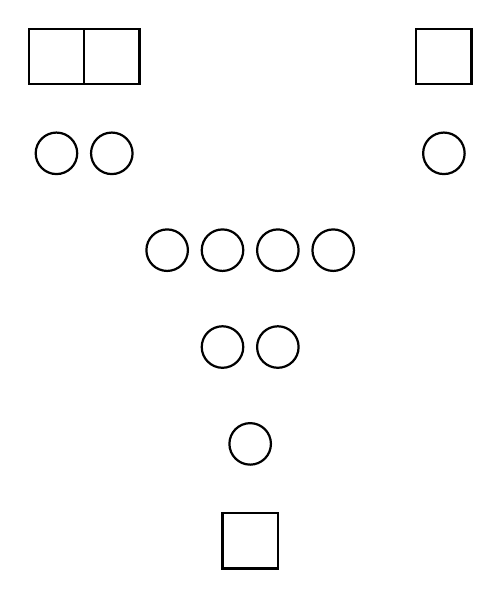
\begin{tikzpicture}

	%% The input row
	\begin{scope}[every node/.style={draw, thick, rectangle, minimum size=2em}]
		\node at ( 0em,0) (1-1) {};
		\node at ( 2em,0) (1-2) {};
		% ...
		\node at (14em,0) (1-8) {};
	\end{scope}

	%% The first row
	%% Shifted down (yshift=-...) and across (xshift=...)
	\begin{scope}[every node/.style={draw, thick, circle, minimum size=1.5em}, yshift=-3.5em]
		\node at ( 0em,0) (2-1) {};
		\node at ( 2em,0) (2-2) {};
		% ...
		\node at (14em,0) (2-8) {};
	\end{scope}

	%% The second row
	%% Shifted down (yshift=-...) and across (xshift=...)
	\begin{scope}[every node/.style={draw, thick, circle, minimum size=1.5em}, xshift=4em, yshift=-7.0em]
		\node at ( 0em,0) (3-1) {};
		\node at ( 2em,0) (3-2) {};
		\node at ( 4em,0) (3-3) {};
		\node at ( 6em,0) (3-4) {};
	\end{scope}

	%% The third row
	\begin{scope}[every node/.style={draw, thick, circle, minimum size=1.5em}, xshift=6em, yshift=-10.5em]
		\node at ( 0em,0) (4-1) {};
		\node at ( 2em,0) (4-2) {};
	\end{scope}

	%% The fourth row
	\begin{scope}[every node/.style={draw, thick, circle, minimum size=1.5em}, xshift=7em, yshift=-14.0em]
		\node at ( 0em,0) (5-1) {};
	\end{scope}

	%% The output row
	\begin{scope}[every node/.style={draw, thick, rectangle, minimum size=2em}, xshift=7em, yshift=-17.5em]
		\node at ( 0em,0) (6-1) {};
	\end{scope}

\end{tikzpicture}
